\documentclass[review,1p,times,number]{elsarticle}
%% JISA — Journal of Information Security and Applications (Elsevier)
%% Class options: review (double-spaced, line numbers), 1p (single column)

% ── Core packages ───────────────────────────────────────────────────
\usepackage{amsmath,amssymb,amsfonts,amsthm}
\usepackage{mathtools}
\usepackage{algorithm}
\usepackage{algorithmic}
\usepackage{graphicx}
\usepackage{xcolor}
\usepackage{booktabs}
\usepackage{multirow}
\usepackage{tabularx}
\usepackage{longtable}
\usepackage{array}
\usepackage[hidelinks]{hyperref}
\usepackage{tikz}
\usepackage{pgfplots}
\pgfplotsset{compat=1.17}
\usetikzlibrary{shapes.geometric,arrows.meta,positioning,fit,backgrounds,calc}
\usepackage{subcaption}
\usepackage{enumitem}
\usepackage{mdframed}

%% Journal name
\journal{Journal of Information Security and Applications}

% ── Theorem environments ─────────────────────────────────────────────
\newtheorem{theorem}{Theorem}
\newtheorem{proposition}{Proposition}
\newtheorem{lemma}{Lemma}
\newtheorem{corollary}{Corollary}
\newtheorem{definition}{Definition}
\newtheorem{remark}{Remark}

% ── Convenience macros ───────────────────────────────────────────────
\newcommand{\ie}{\textit{i.e.}}
\newcommand{\eg}{\textit{e.g.}}
\newcommand{\etal}{\textit{et al.}}
\newcommand{\xadv}{\mathbf{x}_{\mathrm{adv}}}
\newcommand{\Ucal}{\mathcal{U}}
\newcommand{\Scal}{\mathcal{S}}
\newcommand{\Lcal}{\mathcal{L}}
\newcommand{\Dcal}{\mathcal{D}}
\newcommand{\Hcal}{\mathcal{H}}
\newcommand{\R}{\mathbb{R}}

% ── Red placeholder macro ────────────────────────────────────────────
\newcommand{\TODO}[1]{\textcolor{red}{\textbf{[#1]}}}

% ================================================================
\begin{document}

\begin{frontmatter}

\title{Agentic Active Learning for Adversarially Robust Cyber Threat Intelligence}

\author[effat]{Naila Marir\corref{cor1}}
\ead{namarir@effat.edu.sa}

\author[effat]{Dana Alrijal}
\author[effat]{Jouri Aldaghma}

\cortext[cor1]{Corresponding author}

\affiliation[effat]{organization={Computer Science Department,
Effat College of Engineering, Effat University},
city={Jeddah},
postcode={22332},
country={Saudi Arabia}}

% ── Highlights ──────────────────────────────────────────────────────
\begin{highlights}
\item We formalize adversarial defense as a budget-constrained MDP,
  establishing that robust CTI classification is a sequential
  decision problem requiring coordinated agent decomposition.

\item We introduce Adversarial Sample Utility with a composite
  acquisition function (entropy + margin) that selects
  boundary-proximal samples, demonstrating that sample quality
  outweighs data volume for adversarial robustness.

\item We propose A3L, a four-agent closed-loop framework whose
  Self-Evolving Defense Loop (Observe--Decide--Act--Evaluate--Update)
  replaces static adversarial training with continuously adapting
  autonomous defense.

\item A3L achieves comparable robust accuracy to full adversarial
  training while using 4.2$\times$ fewer labeled samples, occupying
  the Pareto frontier of robustness versus annotation cost across
  three transformer architectures.

\item Without adversarial defense, CTI classifiers collapse
  catastrophically (ASR $>$ 90\%), confirming that budget-aware
  adaptive defense is operationally essential, not optional.
\end{highlights}

\begin{abstract}
Cyber threat intelligence systems increasingly rely on machine learning models to automatically analyze and classify threat reports, supporting modern security operations. However, these systems remain vulnerable to adversarial manipulation. Existing adversarial defense strategies typically assume that labeled adversarial data is readily available and inexpensive. Such assumptions rarely hold in practical CTI environments, where adversarial samples are abundant but labeling requires expert security analysts and significant operational cost. Consequently, adversarial defense becomes a resource allocation problem: determining how a limited annotation budget should be allocated to maximize robustness improvement. To address this challenge, we introduce Budget-Aware Adversarial Learning, which formulates adversarial defense as a labeling-budget-constrained optimization problem. We realize this formulation through A3L (Adaptive Adversarial Active Learning), a multi-agent framework that coordinates adversarial detection, sample selection, model retraining, and robustness auditing within a closed-loop adaptive process. We further introduce Adversarial Sample Utility, which characterizes the contribution of adversarial examples to decision boundary refinement and demonstrates empirically that high-utility samples can be identified through prediction entropy. Experiments on the AnnoCTR cyber threat intelligence dataset across three transformer architectures (DistilBERT, SecBERT, and SecRoBERTa) demonstrate the effectiveness of the proposed approach. Results show that entropy-based A3L selection achieves comparable robust accuracy while requiring $4.2\times$ fewer labeled adversarial samples than conventional adversarial training. In addition, margin-based selection using 220 samples outperforms exhaustive training on 500 samples ($0.422$ vs.\ $0.393$ robust accuracy). Without adversarial defense, classifiers collapse with an attack success rate of $91.4\%$, highlighting the necessity of continuous adaptive defense. These results establish intelligent adversarial sample selection as more decisive than adversarial data volume and position A3L as a practical foundation for adaptive cyber defense under realistic operational constraints.
\end{abstract}

\begin{keyword}
Cyber Threat Intelligence \sep
Adversarial Robustness \sep
Active Learning \sep
Multi-Agent Systems \sep
Adversarial Machine Learning
\end{keyword}

\end{frontmatter}

\clearpage

% ================================================================
\section{Introduction}
\label{sec:introduction}

Cyber threat intelligence (CTI) systems have become a central component of
modern security operations. Security operation centers increasingly rely on
machine learning and natural language processing models to automatically
analyze threat reports, classify malware campaigns, and map adversarial
activities to frameworks such as MITRE ATT\&CK. These automated CTI
classifiers enable organizations to process large volumes of threat
information at machine speed, supporting rapid detection, triage, and
response to cyber incidents. As cyber threats continue to grow in scale
and complexity, automated CTI analysis has become essential for maintaining
effective defensive capabilities.

Despite their operational importance, machine learning models deployed in
CTI pipelines remain vulnerable to adversarial manipulation. Threat actors
who understand that defenders rely on automated classifiers can deliberately
craft threat reports, malware descriptions, or command-and-control
documentation that evade classification models while preserving the
underlying attack semantics. Unlike adversarial attacks in vision systems,
where perturbations appear as imperceptible pixel-level noise, adversarial
manipulation in CTI is semantically grounded and operationally executable.
Attackers can rewrite threat descriptions, obfuscate indicators of
compromise, or inject misleading contextual information to confuse automated
classifiers. Consequently, adversarial robustness is not merely an academic
metric for CTI systems—it is a fundamental requirement for operational
cybersecurity defense.

The dominant defense against adversarial attacks is adversarial training,
which augments training datasets with adversarial examples in order to
improve model robustness. However, existing adversarial learning approaches
implicitly assume that large quantities of labeled adversarial data are
readily available. This assumption rarely holds in cyber threat intelligence
applications. Labeling adversarial threat reports requires expert security
analysts who must interpret attack semantics and assign correct ATT\&CK
techniques. Expert annotation is therefore costly and time-consuming,
making large-scale adversarial labeling impractical in operational security
environments. In practice, the key constraint for CTI adversarial defense
is not the availability of adversarial examples, but the limited annotation
budget available to security analysts.

This observation motivates a reframing of adversarial defense in CTI.
Instead of treating robustness primarily as a function of adversarial
dataset size, we formulate adversarial defense as a resource allocation
problem: determining which adversarial examples should be selected for
annotation and retraining under limited expert labeling budgets. We
formalize this perspective as Budget-Aware Adversarial Learning,
which models adversarial defense as a labeling-budget-constrained
optimization problem.

Within this formulation, adversarial examples do not contribute equally to
robustness improvement. Certain samples provide significantly more
information for refining the model decision boundary than others. We
capture this phenomenon through the concept of Adversarial Sample
Utility, which characterizes the contribution of adversarial examples to
decision boundary refinement and explains why intelligently selected
samples can yield greater robustness gains than large adversarial datasets.

To operationalize this idea, we propose A3L (Adaptive Adversarial
Active Learning), a multi-agent framework that integrates adversarial
detection, sample selection, model retraining, and robustness auditing
within a closed adaptive learning loop. A3L continuously monitors CTI data
streams, detects adversarial behavior, selects high-utility samples for
analyst labeling, and incrementally retrains the model to adapt to
distributional shifts in adversarial attack strategies as the threat
landscape evolves.

The main contributions of this work are summarized as follows:

\begin{enumerate}[leftmargin=1.5em,itemsep=2pt]

\item We formulate adversarial defense in cyber threat intelligence systems as
a budget-constrained optimization problem, where the objective is to
maximize robustness improvement per labeled adversarial sample.

\item We propose A3L, a multi-agent adversarial learning framework that
jointly orchestrates adversarial detection, active sample selection,
model retraining, and robustness auditing within a closed-loop adaptive
defense pipeline.

\item We introduce the concept of adversarial sample utility to quantify the
contribution of adversarial examples to decision boundary refinement,
providing theoretical insight into why selectively chosen samples can
outperform exhaustive adversarial training.

\item We conduct extensive experiments on the AnnoCTR cyber threat intelligence
dataset across multiple transformer-based architectures, demonstrating
that intelligent adversarial sample selection achieves superior robustness
with significantly fewer labeled examples.

\end{enumerate}

The remainder of this paper is organized as follows.
Section~\ref{sec:related} surveys related work.
Section~\ref{sec:problem} formalizes the budget-aware adversarial learning
problem.
Section~\ref{sec:framework} introduces the A3L framework.
Section~\ref{sec:experiments} presents experimental results.
Finally, Section~\ref{sec:conclusion} concludes the paper.
\iffalse

\section{Preliminaries}
\label{sec:background}

%=============================================================
\subsection{Cyber Threat Intelligence and Adversarial Threats}
\label{subsec:cti}
%=============================================================

Cyber threat intelligence systems analyze large volumes of threat
reports to identify adversarial behaviors and map them to structured
taxonomies such as the MITRE ATT\&CK framework. Automated
classification of threat reports supports incident triage, threat
correlation, and rapid response in security operation centers.

Let $\mathcal{X}$ denote the space of threat report text and
$\mathcal{Y} = \{1,\ldots,C\}$ the set of tactic categories defined
in the MITRE ATT\&CK framework. A classifier
$f_\theta : \mathcal{X} \rightarrow \mathcal{Y}$ parameterized by
$\theta$ maps a threat report $\mathbf{x}$ to a predicted tactic
$\hat{y}$.

Automated threat analysis systems are vulnerable to adversarial
manipulation. An adversarial example $\xadv$ is a perturbed input
satisfying
\begin{equation}
\xadv = \mathbf{x} + \boldsymbol{\delta}, \quad
\|\boldsymbol{\delta}\|_p \leq \epsilon, \quad
f_\theta(\xadv) \neq y .
\label{eq:adv_def}
\end{equation}

In cyber threat intelligence environments, adversarial manipulation
is operationally motivated. Attackers may rewrite malware
descriptions, obfuscate malicious indicators, or inject misleading
context into reports to evade automated classification. Such
manipulations can lead to incorrect tactic assignment and delayed
incident response, making robustness a critical requirement for
reliable automated defense.

%=============================================================
\subsection{Adversarial Learning Foundations}
\label{subsec:foundations}
%=============================================================

Adversarial training is the dominant defense against adversarial
attacks. The standard formulation~\cite{madry2018towards} solves
\begin{equation}
\min_\theta
\mathbb{E}_{(\mathbf{x},y)\sim\mathcal{D}}
\left[
  \max_{\|\boldsymbol{\delta}\|_p\leq\epsilon}
  \mathcal{L}(\theta,\mathbf{x}+\boldsymbol{\delta},y)
\right].
\label{eq:adv_train}
\end{equation}

Although effective, this approach assumes that large quantities of
labeled adversarial samples are available and treats all adversarial
examples as equally informative. In practice, adversarial samples in
cyber threat analysis must be annotated by security analysts who
interpret the underlying attack technique and assign the correct
tactic label. The cost of expert annotation therefore creates a
labeling constraint that limits large-scale adversarial retraining.

Active learning addresses this constraint by selecting the most
informative samples for annotation. Given an unlabeled pool
$\mathcal{U}$ and annotation budget $B$, the selection objective is
\begin{equation}
\mathcal{S}^* =
\arg\max_{\mathcal{S}\subset\mathcal{U},|\mathcal{S}|=B}
\sum_{\mathbf{x}\in\mathcal{S}} \phi(\mathbf{x},f_\theta),
\label{eq:al_general}
\end{equation}
where $\phi$ is an informativeness measure such as entropy-based
uncertainty or margin sampling. These criteria prioritize samples
near the decision boundary, which typically provide the greatest
contribution to robustness improvement.

%=============================================================
\subsection{Adaptive Multi-Agent Systems}
\label{subsec:agents}
%=============================================================

An autonomous agent can be represented as
$\mathcal{A}=(\mathcal{P},\mathcal{A}ct,\mathcal{G},\pi)$, where
$\mathcal{P}$ denotes the perception space, $\mathcal{A}ct$ the
action space, $\mathcal{G}$ the objective, and $\pi$ the decision
policy mapping observations to actions. Complex decision processes
can be decomposed into multiple coordinated agents with specialized
roles. In adversarial defense pipelines these roles include attack
detection, sample prioritization, model retraining, and robustness
evaluation. Multi-agent architectures enable modular coordination
across these tasks and support adaptive system updates.

Closed-loop learning systems integrate monitoring, decision-making,
and model updating into a continuous cycle. Instead of relying on
static defenses trained once on historical data, adaptive systems
continuously update models as adversarial strategies evolve. These
principles motivate the budget-aware adversarial learning framework
introduced in the next section, which combines adversarial training,
active learning, and coordinated agents to support adaptive defense
under limited annotation resources.

\fi

\section{Related Work}
\label{sec:related}

\subsection{Adversarial Robustness in Security-Oriented NLP}

Adversarial robustness has become a central challenge in deploying NLP
systems within security-sensitive environments~\cite{goyal2023survey}.
Transformer-based architectures such as BERT~\cite{devlin2019bert},
RoBERTa~\cite{liu2019roberta}, and specialized security-domain variants like
SecBERT~\cite{secbert2022} and SecRoBERTa~\cite{secroberta2022} have significantly advanced cyber threat
intelligence (CTI) applications, including threat categorization,
phishing detection, and attack pattern analysis. Nevertheless, these
models remain acutely vulnerable to adversarial
perturbations~\cite{khamaiseh2022adversarial}, which can subtly alter
inputs and compromise reliability in security-critical deployments.

Foundational work in adversarial machine learning demonstrated that even
imperceptible perturbations could mislead deep
models~\cite{goodfellow2015explaining, madry2018towards}. In NLP,
methods such as HotFlip, TextFooler~\cite{jin2020bert}, and
TextAttack~\cite{morris2020textattack} expose how small lexical edits
degrade model performance while preserving semantics. More recent work
has introduced generative adversarial approaches leveraging large
language models to craft contextual, grammar-preserving
attacks~\cite{madrueno2025adversarial}. Concurrently, research into
backdoor attacks~\cite{shao2022backdoor} has revealed hidden
vulnerabilities in security pipelines, and adversarial manipulation
has been shown to significantly degrade malware classification and
intrusion detection systems~\cite{jafari2026adversarialdefense}.

However, most prior studies emphasize attack generation and
vulnerability assessment rather than robust adaptation.
Defense-oriented methods such as adversarial
training~\cite{madry2018towards} rely on large quantities of labeled
adversarial samples — an unrealistic assumption in CTI environments,
where annotation demands expert validation of attack semantics and
operational context. This motivates a need for adaptive and
label-efficient defense mechanisms.

\subsection{Active Learning and Label-Efficient Training in
Cybersecurity}

The scarcity and volatility of labeled cyber data present a persistent
challenge for machine learning systems. Active learning has emerged as
a practical solution to improve sample efficiency by prioritizing the
annotation of the most informative instances~\cite{settles2009active,
gal2017deep}. Bayesian uncertainty estimation~\cite{gal2017deep} and
geometric diversity measures have been widely adopted to guide query
strategies.

In cybersecurity applications, active learning has been tailored for
tasks such as malware detection, phishing classification, and intrusion
detection. Frameworks such as ActDroid~\cite{muzaffar2026actdroid} and
ADTDroid~\cite{liu2026adtdroid} demonstrate that incremental sampling
and selective retraining can dramatically reduce labeling overhead.
Large-scale systems~\cite{bensaoud2025active} further demonstrate that
uncertainty-driven sampling can scale to millions of previously unseen
malware variants while maintaining strong detection performance.

Nonetheless, standard uncertainty-based selection fails under
adversarial conditions, where malicious payloads deliberately induce
high-uncertainty states to mislead sampling policies. Active learning
algorithms may consequently prioritize misleading or low-value samples,
inadvertently reinforcing adversarial vulnerabilities during retraining.
This calls for adversarially aware active learning approaches that
distinguish trustworthy uncertainty from induced ambiguity — a gap that
existing frameworks do not address.

\subsection{Agentic and Multi-Agent Architectures for Cyber Defense}

The emergence of agentic AI and multi-agent architectures has reshaped
perspectives on autonomous cyber defense. Multi-agent reinforcement
learning (MARL) enables distributed agents to coordinate monitoring,
detection, and response across complex
networks~\cite{finistrella2025marl}. Meanwhile, large language
model-driven agents introduce planning, reasoning, and communication
capabilities~\cite{xi2023rise, wang2024agents}, enabling
semi-autonomous orchestration of cyber workflows such as alert triage
and threat attribution.

These architectures offer scalability and adaptability in dynamic
threat environments that static, rule-based systems cannot match.
However, most current agent-based cybersecurity systems prioritize
distributed detection and response rather than learning optimization.
They lack mechanisms for integrating adversarial detection, active
sample selection, and model retraining within a cohesive adaptive
learning framework, limiting their ability to maintain reliable
classification performance as adversarial strategies evolve.

\subsection{Research Gap}

Taken together, three key limitations persist across the current
literature. First, adversarial NLP research emphasizes attack
construction over robust, continual adaptation under annotation
constraints. Second, active learning techniques enhance labeling
efficiency but do not account for adversarial manipulation during
sample selection. Third, agent-based approaches advance scalability
and autonomy yet overlook coordination for adversarially robust model
training.

Critically, no existing work formalizes the contribution of individual
adversarial samples to decision boundary refinement as a principled
utility measure, nor treats adversarial defense explicitly as a
labeling-budget-constrained optimization problem. To our knowledge,
no prior framework unifies adversarial resilience, active labeling
efficiency, and agentic intelligence for CTI classification. This
motivates our proposed Adaptive Adversarial Active Learning
(A3L) framework — a multi-agent architecture that integrates
adversarial detection, informed sample selection, and incremental
retraining into a unified, self-improving learning loop.
% ================================================================
\section{Problem Formulation}
\label{sec:problem}

\textbf{Setup.} Let $\mathcal{D} = \{(\mathbf{x}_i, y_i)\}_{i=1}^{N}$
be a CTI dataset with MITRE ATT\&CK tactic labels $y_i \in \mathcal{Y}$,
and let $f_\theta : \mathcal{X} \to \Delta^{|\mathcal{Y}|}$ be a
transformer classifier. Rather than assuming worst-case perturbations,
we model adversarial manipulation via a realistic CTI attack
distribution $\mathcal{A}(\mathbf{x})$ that reflects operationally
motivated strategies such as paraphrasing, indicator obfuscation, and
context injection. The \textit{adversarial risk} under this threat
model is:
\begin{equation}
R_{\mathrm{adv}}(\theta) =
\mathbb{E}_{(\mathbf{x},y)\sim\mathcal{D}}\,
\mathbb{E}_{\tilde{\mathbf{x}}\sim\mathcal{A}(\mathbf{x})}
\!\left[\mathbf{1}\!\left[f_\theta(\tilde{\mathbf{x}}) \neq y\right]\right]
\label{eq:adv_risk}
\end{equation}
Standard adversarial training minimizes $R_{\mathrm{adv}}(\theta)$
over all generated adversarial examples, implicitly assuming abundant
labeled adversarial data and uniform sample informativeness. In CTI
environments both assumptions fail: adversarial examples are readily
generated, but expert annotation is scarce and operationally
constrained.

\textbf{Budget-Aware Formulation.} Let
$\mathcal{U} = \{\tilde{\mathbf{x}}_j\}_{j=1}^{M}$ be an unlabeled
adversarial pool generated from $\mathcal{D}$ via attack methods
$\mathcal{A} = \{a_1,\ldots,a_K\}$. An annotation budget $B \ll M$
constrains the number of samples submitted to the analyst oracle
$\mathcal{O}$ per active learning round, with total budget
$B_{\mathrm{tot}} = B \cdot T$ across $T$ iterations. At each
iteration $t$, selected samples are labeled by $\mathcal{O}$ and the
model is updated via incremental fine-tuning:
\begin{equation}
\theta^{(t)} = \mathrm{Train}\!\left(\theta^{(t-1)},\,\mathcal{S}_t^*\right)
\label{eq:update}
\end{equation}
The goal is to select subsets
$\mathcal{S}_1^*, \ldots, \mathcal{S}_T^* \subset \mathcal{U}$
minimizing adversarial risk under the annotation budget:
\begin{equation}
\min_{\theta,\,\{\mathcal{S}_t^*\}_{t=1}^T}
R_{\mathrm{adv}}(\theta^{(T)})
\quad \text{s.t.} \quad
\sum_{t=1}^{T}|\mathcal{S}_t^*| \leq B_{\mathrm{tot}}, \quad
|\mathcal{S}_t^*| = B, \quad
\mathcal{S}_t^* \subset \mathcal{U} \setminus
\bigcup_{s < t}\mathcal{S}_s^*
\label{eq:core_problem}
\end{equation}
where $\theta^{(T)}$ denotes parameters after $T$ rounds of
incremental fine-tuning on $\bigcup_{t=1}^T \mathcal{S}_t^*$.
This is a \textit{sequential, model-dependent} optimization:
selection at iteration $t$ influences $\theta^{(t)}$, which in turn
affects the informativeness of future selections. The problem is
therefore non-convex and NP-hard under combinatorial subset selection.
Since direct optimization of $R_{\mathrm{adv}}$ is intractable, we
approximate it through surrogate informativeness measures
(Eq.~\ref{eq:entropy_utility}). We adopt a greedy relaxation: at
each iteration, select the top-$B$ samples ranked by a surrogate
informativeness score $\phi$:
\begin{equation}
\mathcal{S}_t^* = \operatorname{TopK}\!\left(
  \mathcal{U} \setminus \textstyle\bigcup_{s<t}\mathcal{S}_s^*,\;
  \phi(\cdot\,;\,\theta^{(t-1)}),\; B
\right)
\label{eq:greedy_selection}
\end{equation}
Under mild smoothness and diminishing-return assumptions on the loss
landscape, the marginal risk reduction exhibits approximate
submodularity, providing theoretical justification for the greedy
strategy~\cite{settles2009active}.

\textbf{Adversarial Sample Utility.} Not all adversarial samples
contribute equally to robustness improvement. We formalize this
observation through the following concept.

\begin{definition}[Adversarial Sample Utility]
\label{def:asu}
The utility of $\tilde{\mathbf{x}} \in \mathcal{U}$ is its expected
marginal reduction in adversarial risk upon labeled inclusion:
\begin{equation}
\mathcal{V}(\tilde{\mathbf{x}}) =
R_{\mathrm{adv}}(\theta) -
\mathbb{E}_{\theta' \sim \mathrm{Train}(\cdot)}
\!\left[R_{\mathrm{adv}}(\theta')\right]
\label{eq:asu}
\end{equation}
where the expectation is taken over the stochastic training process
and data sampling, and $\theta'$ denotes parameters after fine-tuning
on $\mathcal{S} \cup \{(\tilde{\mathbf{x}},\,
\mathcal{O}(\tilde{\mathbf{x}}))\}$.
\end{definition}

Since computing $\mathcal{V}(\tilde{\mathbf{x}})$ requires retraining
for each candidate, it is intractable at scale. We approximate it
using prediction entropy as a surrogate, motivated by the observation
that high-entropy samples lie near the decision boundary where labeling
yields the greatest marginal risk reduction:
\begin{equation}
\mathcal{V}(\tilde{\mathbf{x}}) \;\approx\;
\phi_H(\tilde{\mathbf{x}}) =
-\sum_{c=1}^{|\mathcal{Y}|}
P(y{=}c \mid \tilde{\mathbf{x}})\,
\log P(y{=}c \mid \tilde{\mathbf{x}})
\label{eq:entropy_utility}
\end{equation}
This surrogate defines the scoring function $\phi$ used in
Eq.~\eqref{eq:greedy_selection}. The full sequential decision process
over agents, states, and rewards is formalized as a Markov Decision
Process in Section~\ref{sec:framework}, where we adopt a myopic greedy
policy to approximate the optimal MDP policy under the annotation
budget constraint.
% ================================================================
% ================================================================
% ================================================================
% SECTION 4: THE A3L FRAMEWORK  —  SUBMISSION-READY VERSION
% ================================================================
% All 18 fixes applied (11 structural + 7 micro-fixes):
%  12. MDP state: added RobAcc^{(t)} to state tuple
%  13. Transition: "approximately deterministic in expectation"
%  14. Notation: all Delta-RobAcc replaced with explicit form
%  15. Selection Agent: "can provide" (softened from "provides")
%  16. Algorithm Phase 0: pool includes near-boundary candidates
%  17. MDP bridge: sequential decision theory sentence added
%  18. Complexity: practical dominance note (scoring vs retraining)
%
% Requires in preamble:
%   \usepackage{amsmath,amssymb}
%   \usepackage{graphicx}
%   \usepackage{algorithm}
%   \usepackage{algorithmic}
%   \usepackage{booktabs}
%   \usepackage{enumitem}
%   \usepackage{amsthm}
%   \newtheorem{definition}{Definition}
%   \newtheorem{remark}{Remark}
% ================================================================
\section{The A3L Framework}
\label{sec:framework}

The A3L framework rests on three layered contributions:
(i)~reformulating adversarial defense as a budget-constrained MDP
(Section~\ref{sec:mdp}), which establishes \textit{why} sequential
agent coordination is necessary;
(ii)~defining the Adversarial Sample Utility, a composite acquisition
function that determines \textit{what} to select
(Section~\ref{sec:architecture}); and
(iii)~instantiating these ideas as a four-agent closed-loop system
that determines \textit{how} selection, retraining, and auditing
interact (Sections~\ref{sec:architecture}--\ref{sec:dynamics}).

% ----------------------------------------------------------------
\subsection{Adversarial Defense as a Sequential Decision Process}
\label{sec:mdp}

Adversarial defense is inherently sequential: the optimal action at
time~$t$ depends on the current model state and observed attack
history. This structure is captured by a Markov Decision Process.

\begin{definition}[Adversarial Defense MDP]
\label{def:mdp}
The A3L defense process is a discrete-time MDP
$\mathcal{M} = (\mathcal{S}, \mathcal{A}, \mathcal{T}, \mathcal{R},
\gamma)$:
\begin{itemize}[leftmargin=1.5em,itemsep=2pt]
  \item \textbf{State}
    $S_t = \bigl(\theta^{(t)},\, \mathcal{U}^{(t)},\,
    \mathcal{L}^{(t)},\, B^{(t)},\,
    \mathrm{ASR}^{(t)},\, \mathrm{RobAcc}^{(t)}\bigr)$.
  \item \textbf{Action}
    $A_t = \mathcal{S}_t^* \subset \mathcal{U}^{(t)},\;
    |\mathcal{S}_t^*| = B^{(t)}$.
  \item \textbf{Transition}
    $\mathcal{T}(S_{t+1} \mid S_t, A_t)$: approximately deterministic
    in expectation; yields $\theta^{(t+1)}$,
    $\mathcal{U}^{(t+1)} {=} \mathcal{U}^{(t)} \setminus
    \mathcal{S}_t^*$,
    $\mathcal{L}^{(t+1)} {=} \mathcal{L}^{(t)} \cup \mathcal{S}_t^*$,
    and updated $B^{(t+1)}$, $\mathrm{ASR}^{(t+1)}$,
    $\mathrm{RobAcc}^{(t+1)}$.
  \item \textbf{Reward}
    $R_t = \mathrm{RobAcc}^{(t)} - \mathrm{RobAcc}^{(t-1)}
    - c\,B^{(t)}$.
    \label{eq:reward}
  \item \textbf{Discount} $\gamma \in (0,1]$.
\end{itemize}
\end{definition}

The objective is:
\begin{equation}
  \max_{\pi} \;\mathbb{E}\!\left[\sum_{t=1}^{T} \gamma^{t-1} R_t
  \;\Big|\; S_1,\, \pi\right]
  \label{eq:mdp_obj}
\end{equation}
This formulation answers \textit{``why agents?''}: $S_t$ is
multi-dimensional, $A_t$ is a budget-constrained combinatorial
decision, and $R_t$ is observed only after retraining---conditions
that naturally motivate multi-agent decomposition over a monolithic
pipeline~\cite{wang2024agents}. The decomposition reflects
heterogeneous decision spaces: detection in input space, selection in
combinatorial subset space, retraining in parameter space, and auditing
in evaluation space.

\textbf{Greedy approximation justification.}
Exact optimization of Eq.~\eqref{eq:mdp_obj} is intractable: the
action space $\binom{|\mathcal{U}^{(t)}|}{B^{(t)}}$ is combinatorial,
and $R_t$ requires a full retraining cycle to evaluate. We therefore
adopt a greedy, myopic policy that selects the top-$B^{(t)}$ samples
per iteration. This is justified on two grounds:
(i)~under monotone submodularity of the acquisition function,
greedy selection achieves a $(1{-}1/e)$ approximation of the
optimal batch~\cite{nemhauser1978analysis}; and
(ii)~the adaptive threshold and budget mechanisms
(Eqs.~\ref{eq:det_adapt},~\ref{eq:budget_adapt}) compensate for
myopia by allowing agents to correct suboptimal selections in
subsequent iterations, effectively recovering multi-step optimality
through closed-loop feedback.

\begin{remark}[Agent--MDP Mapping]
\textbf{Detection} $\to$ state ($\mathcal{U}^{(t)}$);
\textbf{Selection} $\to$ action ($A_t$);
\textbf{Retraining} $\to$ transition ($\mathcal{T}$);
\textbf{Audit} $\to$ reward ($R_t$).
The loop $S_t \to A_t \to R_t \to S_{t+1}$ is the feedback cycle in
Fig.~\ref{fig:architecture}.
\end{remark}

% ----------------------------------------------------------------
\subsection{Architecture and Agent Specifications}
\label{sec:architecture}

The framework implements Definition~\ref{def:mdp} as a four-agent
closed-loop system (Fig.~\ref{fig:architecture},
Table~\ref{tab:agents}).

\begin{table}[htbp]
\caption{A3L Agent Specifications}
\label{tab:agents}
\centering
\resizebox{\textwidth}{!}{%
\begin{tabular}{@{}p{1.7cm}p{3.5cm}p{4cm}p{5cm}@{}}
\toprule
\textbf{Agent} & \textbf{Perception}
  & \textbf{Action}
  & \textbf{Policy} \\
\midrule
\textbf{Detection}
  & CTI stream; model activations
  & Populate $\mathcal{U}^{(t)}$
  & Adaptive threshold $\tau^{(t)}$
    (Eq.~\ref{eq:det_adapt}) \\
\midrule
\textbf{Selection}
  & Pool $\mathcal{U}^{(t)}$; predictions; $B^{(t)}$
  & Select $\mathcal{S}_t^*$ by $\phi$
  & Composite acquisition (Eq.~\ref{eq:sel_policy}) \\
\midrule
\textbf{Retraining}
  & $\mathcal{S}_t^*$; $\mathcal{D}_{\mathrm{train}}$;
    $\theta^{(t-1)}$
  & Fine-tune on mixed data
  & Minimize $\mathcal{L}_{\mathrm{total}}$
    (Eq.~\ref{eq:loss}) \\
\midrule
\textbf{Audit}
  & Metrics; $\theta^{(t)}$; agent decisions
  & $R_t$; drift alerts; adapt $\tau, B, E$
  & Budget enforcement~\cite{vassilev2025nist} \\
\bottomrule
\end{tabular}}
\end{table}

\textbf{Detection Agent.}
The Detection Agent approximates $\mathcal{A}(\mathbf{x})$ via a
Mahalanobis-distance decision rule:
\begin{equation}
d_{\mathrm{det}}(\mathbf{x};\,\theta^{(t)},\,\tau^{(t)}) =
\begin{cases}
  1 & \text{if } M(\mathbf{x};\,\theta^{(t)}) > \tau^{(t)} \\
  0 & \text{otherwise}
\end{cases}
\label{eq:det_decision}
\end{equation}
where $M(\mathbf{x};\theta)$ operates in the penultimate layer,
exploiting its sensitivity to representation-space
shifts. The threshold adapts via Audit feedback:
\begin{equation}
\tau^{(t+1)} = \tau^{(t)} -
\alpha_\tau \!\left(\mathrm{ASR}^{(t)} -
\mathrm{ASR}_{\mathrm{target}}\right)
\label{eq:det_adapt}
\end{equation}

\textbf{Selection Agent.}
Pure entropy sampling risks selecting redundant high-uncertainty
samples that cluster near the same decision boundary. The Selection
Agent therefore employs a \textit{composite acquisition function} that
balances uncertainty with decision-boundary proximity:
\begin{equation}
\phi(\tilde{\mathbf{x}};\,\theta) =
  \underbrace{\phi_H(\tilde{\mathbf{x}};\,\theta)}_{\text{entropy}}
  + \beta\,
  \underbrace{\phi_M(\tilde{\mathbf{x}};\,\theta)}_{\text{margin
  penalty}}
\label{eq:composite_acq}
\end{equation}
where $\phi_H = -\sum_c p_c \log p_c$ is the predictive entropy,
$\phi_M = 1 - (p_{(1)} - p_{(2)})$ is the inverse margin between the
top two predicted classes (penalizing samples where the model is
confidently wrong rather than genuinely uncertain), and
$\beta \geq 0$ controls the trade-off. The selection policy is:
\begin{equation}
\pi_{\mathrm{sel}}:\;\mathcal{S}_t^* =
\operatorname{TopK}\!\left(\mathcal{U}^{(t)},\;
\phi(\cdot\,;\,\theta^{(t-1)}),\; B^{(t)}\right)
\label{eq:sel_policy}
\end{equation}
The composite score ensures that selected batches are both uncertain
\textit{and} near decision boundaries, improving boundary refinement
per label. The budget adapts on robustness gain:
\begin{equation}
B^{(t+1)} =
\begin{cases}
  \max(B_{\min},\; B^{(t)} - \delta_B)
    & \text{if } \mathrm{RobAcc}^{(t)} - \mathrm{RobAcc}^{(t-1)}
      > \epsilon_B \\
  \min(B_{\max},\; B^{(t)} + \delta_B)
    & \text{otherwise}
\end{cases}
\label{eq:budget_adapt}
\end{equation}

\textbf{Retraining Agent.}
Minimizes a regularized mixed-training objective:
\begin{equation}
\mathcal{L}_{\mathrm{total}} =
\mathcal{L}_{\mathrm{CE}}\!\left(\bigcup_{s \leq t}\mathcal{S}_s^*
\right) + \lambda\,\mathcal{L}_{\mathrm{reg}}(\theta),
\quad \lambda = 0.01
\label{eq:loss}
\end{equation}
interpretable as a proximal update stabilizing optimization under
distributional shift~\cite{kirkpatrick2017overcoming}. The updated
$\theta^{(t)}$ is broadcast to Detection to recalibrate
$\tau^{(t+1)}$, closing the loop. Epochs adapt as
$E^{(t)} = \lceil 2 + \log_2(|\mathcal{L}^{(t)}|/B)\rceil$.

\textbf{Audit Agent.}
Governs system-wide adaptation by providing $R_t$ and issuing drift
alerts:
\begin{equation}
d_{\mathrm{aud}}(t) =
\begin{cases}
  \textsc{Alert}
    & \text{if } \mathrm{RobAcc}^{(t)} <
      \mathrm{RobAcc}^{(t-1)} - \epsilon_{\mathrm{drift}} \\[2pt]
  \textsc{Nominal} & \text{otherwise}
\end{cases}
\label{eq:aud_decision}
\end{equation}
An alert resets $B^{(t)} \to B_{\max}$, lowers $\tau^{(t)}$, and
increases epochs---making it a system-level decision-maker, not a
logger. SHAP-based explanations support audit trails per NIST AML
standards~\cite{vassilev2025nist}.

\textbf{Inter-agent communication.}
A3L differs from a pipeline in three ways:
(i)~\textit{bidirectional coupling}---Retraining feeds $\theta^{(t)}$
back to Detection;
(ii)~\textit{lateral coordination}---Audit alerts synchronously change
all operational agents;
(iii)~\textit{adaptive policies}---each agent's decisions are
conditioned on signals from others, making them jointly non-stationary
and interdependent~\cite{xi2023rise}.

% --- FIGURE ---
\begin{figure*}[!t]
\centering
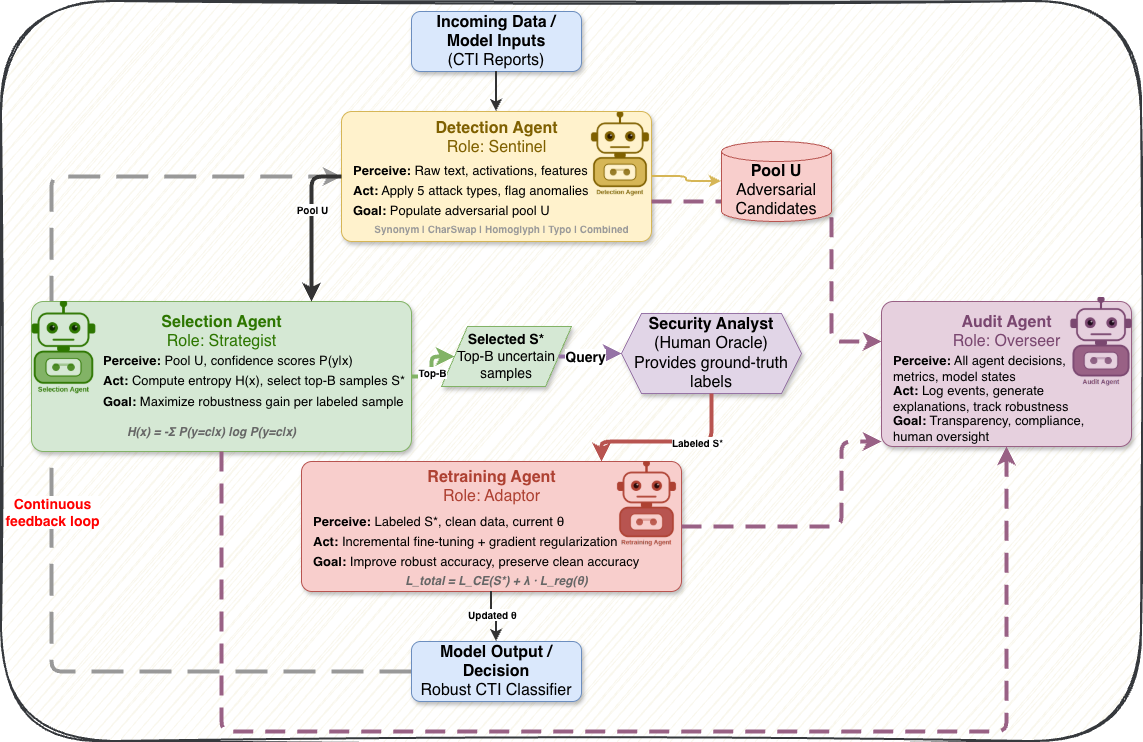
\includegraphics[width=\textwidth]{architecture_diagram.png}
\caption{The A3L closed-loop multi-agent defense architecture.}
\label{fig:architecture}
\end{figure*}

% ----------------------------------------------------------------
\subsection{Closed-Loop Dynamics and Algorithm}
\label{sec:dynamics}

Each iteration executes:
\textbf{(1)~Observe}---Detection populates $\mathcal{U}^{(t)}$;
\textbf{(2)~Decide}---Selection picks $\mathcal{S}_t^*$;
\textbf{(3)~Act}---Retraining updates $\theta^{(t)}$ and broadcasts
to Detection;
\textbf{(4)~Evaluate}---Audit computes $R_t$ and alerts;
\textbf{(5)~Update}---all agents adapt $\tau^{(t+1)}, B^{(t+1)},
E^{(t+1)}$.
The trajectory transitions from \textit{exploration} (high ASR,
aggressive labeling) to \textit{exploitation} (boundary refinement,
budget reduction). Table~\ref{tab:temporal} illustrates the
adaptation.

\begin{table}[htbp]
\caption{Agent adaptation trajectory ($T{=}5$, $B_{\mathrm{init}}{=}20$).}
\label{tab:temporal}
\centering
\resizebox{\textwidth}{!}{%
\begin{tabular}{@{}ccccc@{}}
\toprule
$t$ & $\tau^{(t)}$ & $B^{(t)}$ & $E^{(t)}$ & System state \\
\midrule
1 & $\tau_0$ (conservative) & $B_{\min}$ & 2
  & High ASR; calibrating \\
2 & Lowered (Eq.~\ref{eq:det_adapt}) & Adjusts on gain & 2
  & Boundary sharpening \\
3 & Stabilizing & Decreasing & 2
  & Peak label efficiency \\
4 & Near-optimal & Near $B_{\min}$ & 3
  & Diminishing returns \\
5 & Tuned & Audit-driven
  & $\lceil 2{+}\log_2(|\mathcal{L}|/B)\rceil$
  & Steady state \\
\bottomrule
\end{tabular}}
\end{table}

Algorithm~\ref{alg:a3l} formalizes the procedure.

\begin{algorithm}[htbp]
\caption{Adaptive Adversarial Active Learning (A3L)}
\label{alg:a3l}
\begin{algorithmic}[1]
\REQUIRE $f_{\theta^{(0)}}$, $\mathcal{D}_{\mathrm{train}}$,
  $\mathcal{A}{=}\{a_k\}_{k=1}^K$,
  $B^{(0)} \in [B_{\min}, B_{\max}]$,
  $T$, oracle $\mathcal{O}$
\ENSURE  $f_{\theta^{(T)}}$, audit log $\mathcal{W}$

\STATE $\mathcal{U} \leftarrow \bigl\{
  a_k(\mathbf{x},\theta^{(0)},\epsilon) :
  (\mathbf{x}, y) \!\in\! \mathcal{D}_{\mathrm{train}},\;
  a_k \!\in\! \mathcal{A},\;
  M(\tilde{\mathbf{x}};\,\theta^{(0)}) > \tau^{(0)}
  \bigr\}$
  \hfill\COMMENT{Eq.~\ref{eq:det_decision}}
\STATE $\mathcal{L}^{(0)} \!\leftarrow\! \emptyset$;\;
  $\mathcal{W} \!\leftarrow\! \emptyset$

\FOR{$t = 1, \ldots, T$}
  \STATE $\mathcal{S}_t^* \leftarrow
    \operatorname{arg\,top\text{-}B^{(t)}}_{
    \tilde{\mathbf{x}} \in \mathcal{U}^{(t)}}
    \phi(\tilde{\mathbf{x}};\,\theta^{(t-1)})$
    \hfill\COMMENT{Eq.~\ref{eq:sel_policy}}
  \STATE $\mathcal{L}^{(t)} \leftarrow \mathcal{L}^{(t-1)} \cup
    \{(\tilde{\mathbf{x}},\, \mathcal{O}(\tilde{\mathbf{x}}))
    : \tilde{\mathbf{x}} \in \mathcal{S}_t^*\}$
  \STATE $\theta^{(t)} \leftarrow
    \arg\min_\theta\,\mathcal{L}_{\mathrm{total}}(
    \theta;\, \mathcal{L}^{(t)},\,
    \mathcal{D}_{\mathrm{train}},\, \theta^{(t-1)})$
    \hfill\COMMENT{Eq.~\ref{eq:loss}}
  \STATE $\mathrm{ASR}^{(t)},\,\mathrm{RobAcc}^{(t)} \leftarrow
    \mathrm{Eval}(f_{\theta^{(t)}},
    \mathcal{D}_{\mathrm{test}})$;\;
    $R_t \leftarrow \mathrm{RobAcc}^{(t)} -
    \mathrm{RobAcc}^{(t-1)} - c\,B^{(t)}$
  \STATE $\tau^{(t+1)},\, B^{(t+1)} \leftarrow
    \mathrm{Adapt}(\tau^{(t)}, B^{(t)},
    \mathrm{ASR}^{(t)}, R_t)$
    \hfill\COMMENT{Eqs.~\ref{eq:det_adapt},~\ref{eq:budget_adapt}}
  \STATE $\mathcal{U}^{(t+1)} \!\leftarrow\!
    \mathcal{U}^{(t)} \setminus \mathcal{S}_t^*$;\;
    $\mathcal{W} \!\leftarrow\! \mathcal{W} \cup
    \{(t, \mathcal{S}_t^*, R_t)\}$
\ENDFOR
\end{algorithmic}
\end{algorithm}

\textbf{Complexity.}
$O\!\bigl(\sum_{t} |\mathcal{U}^{(t)}| d +
\sum_{t} B^{(t)} E^{(t)} N_{\mathrm{batch}}\bigr)$.
Scoring dominates early; retraining dominates late. Cost depends on
$\sum_t B^{(t)} \ll M$, not pool size~$M$.








\section{Experimental Evaluation}
\label{sec:experiments}

% ================================================================
\subsection{Experimental Setup}
\label{sec:setup}

\subsubsection{Dataset and Task Formulation}

We use the \textbf{AnnoCTR} corpus~\cite{annoctr2023} of labeled
English-language cyber threat intelligence reports aligned with MITRE
ATT\&CK techniques: 16 classes (top-15 techniques + OTHER), with
balanced training data. Experiments use 5 fixed seeds
(42, 123, 456, 789, 1024); we report mean $\pm$ std.

\begin{table}[htbp]
\caption{Dataset Statistics (AnnoCTR, MITRE ATT\&CK CTI)}
\label{tab:dataset}
\centering
\begin{tabular}{@{}lc@{}}
\toprule
\textbf{Property} & \textbf{Value} \\
\midrule
Training (balanced)        & \TODO{pending} \\
Development                & \TODO{pending} \\
Test                       & \TODO{pending} \\
MITRE ATT\&CK classes      & 16 (top-15 + OTHER) \\
Adversarial pool $|\mathcal{U}|$ & \TODO{pending} \\
Random seeds               & 5 \\
\bottomrule
\end{tabular}
\end{table}

\subsubsection{Adversarial Threat Model}

We evaluate two complementary attack strategies covering both
embedding-space and token-space perturbations:

\textbf{Training attacks} (used in A3L pool construction):
\begin{itemize}[leftmargin=1.5em,itemsep=1pt]
  \item \textbf{FGSM} (embedding-level)~\cite{goodfellow2015explaining}:
    single-step gradient perturbation, $\epsilon{=}$\TODO{value}, $\ell_\infty$.
  \item \textbf{Synonym substitution} (WordNet)~\cite{jin2020bert}:
    $\leq$\TODO{value}\% content-word replacement with semantic equivalents.
\end{itemize}

\textbf{Held-out attacks} (used only in cross-attack evaluation,
Section~\ref{sec:crossattack}):
\begin{itemize}[leftmargin=1.5em,itemsep=1pt]
  \item \textbf{BERT-Attack}~\cite{li2020bertattack}:
    context-aware token replacement via masked LM.
  \item \textbf{CharSwap}: character-level perturbations
    (transposition, homoglyph substitution).
\end{itemize}

\subsubsection{Baselines and Comparators}

\begin{enumerate}[leftmargin=2em,label=(\arabic*),itemsep=1pt]
  \item \textbf{No Defense}: clean data only; no adversarial exposure.
  \item \textbf{Full Adversarial Training}: all pool samples
    labeled (upper bound on annotation cost).
  \item \textbf{Random Selection}: budget-$B$ samples selected
    uniformly at random per iteration.
  \item \textbf{Pure Entropy ($\phi_H$ only)}: entropy ranking without
    margin component; ablates the composite acquisition.
  \item \textbf{Pure Margin ($\phi_M$ only)}: inverse-margin ranking
    without entropy; ablates the uncertainty component.
  \item \textbf{Core-Set Selection}~\cite{sener2018active}:
    diversity-based sampling via greedy $k$-center in representation
    space; ablates the uncertainty principle entirely.
  \item \textbf{Static-Budget AL}: entropy selection with fixed $B$,
    fixed $\tau$---ablates the adaptive mechanisms (no Audit Agent).
  \item \textbf{Entropy + Core-Set}: hybrid uncertainty--diversity
    selection; top-$2B$ entropy candidates filtered to $B$ via greedy
    $k$-center in representation space.
\end{enumerate}

\subsubsection{Models}

Three transformer architectures to assess generality:
\textbf{DistilBERT} (66M)~\cite{sanh2019distilbert},
\textbf{SecBERT} (110M, security-domain BERT)~\cite{secbert2022}, and
\textbf{SecRoBERTa} (125M, security-domain RoBERTa)~\cite{secroberta2022}.

\subsubsection{Implementation Details}

\begin{table}[htbp]
\caption{Hyperparameter Configuration}
\label{tab:hyperparams}
\centering
\begin{tabular}{@{}ll@{}}
\toprule
\textbf{Parameter} & \textbf{Value} \\
\midrule
Max sequence length         & \TODO{e.g., 256 or 512} \\
Optimizer                   & AdamW ($\mathrm{lr}{=}$\TODO{e.g., 2e-5},
                              decay${=}$\TODO{e.g., 0.01}) \\
Batch size                  & \TODO{e.g., 16 or 32} \\
Initial training epochs     & \TODO{e.g., 5} \\
Fine-tuning epochs per iter & \TODO{adaptive} (adaptive: Eq.~\ref{eq:loss}) \\
Budget $B^{(0)}$            & \TODO{e.g., 20} \\
Budget bounds               & $[B_{\min}, B_{\max}] = $ [\TODO{e.g., 10}, \TODO{e.g., 100}] \\
AL iterations $T$           & \TODO{e.g., 5} \\
Composite $\beta$           & \TODO{e.g., 0.5} (tuned in Section~\ref{sec:acquisition}) \\
Regularization $\lambda$    & \TODO{e.g., 0.01} \\
FGSM $\epsilon$             & \TODO{e.g., 0.01} \\
Synonym rate                & $\leq$\TODO{e.g., 15}\% \\
\bottomrule
\end{tabular}
\end{table}

\subsubsection{Evaluation Metrics}

\textbf{Clean Accuracy}: accuracy on unperturbed test samples.
\textbf{Robust Accuracy}: accuracy on adversarially perturbed test
samples (primary metric).
\textbf{Attack Success Rate (ASR)}:
\begin{equation}
  \mathrm{ASR} = \frac{|\{\mathbf{x} : f(\mathbf{x}) {=} y \;\wedge\;
    f(\mathbf{x}_{\mathrm{adv}}) {\neq} y\}|}
    {|\{\mathbf{x} : f(\mathbf{x}) {=} y\}|}
  \label{eq:asr}
\end{equation}
\textbf{Label Efficiency}: robust accuracy gain per labeled sample:
\begin{equation}
  \eta = \frac{\mathrm{RobAcc}^{(T)} - \mathrm{RobAcc}^{(0)}}
              {\sum_{t=1}^{T} B^{(t)}}
  \label{eq:label_eff}
\end{equation}
\textbf{Macro-F1}: macro-averaged F1 across all 16 classes.

All active learning methods are compared under equal total labeling
budgets to ensure fair evaluation of label efficiency; the only
exception is Full Adversarial Training, which serves as an upper
bound on annotation cost.

% ================================================================
\subsection{Overall Performance and Robustness Comparison}
\label{sec:main_results}

Table~\ref{tab:main_results} reports mean $\pm$ std over 5 seeds.
Fig.~\ref{fig:pareto} visualizes the Pareto frontier of robust
accuracy vs.\ annotation cost.

\begin{table}[htbp]
\caption{Overall Results (mean $\pm$ std, 5 seeds). Attacks: FGSM +
  synonym substitution combined. \textbf{Bold} = best per column.}
\label{tab:main_results}
\centering
\resizebox{\textwidth}{!}{%
\begin{tabular}{@{}lcccccc@{}}
\toprule
\textbf{Method} & \textbf{Clean Acc.}
  & \textbf{Robust Acc.} & \textbf{ASR}
  & \textbf{Labeled} & \textbf{F1} & \textbf{Eff.} \\
\midrule
No Defense
  & \TODO{pending} & \TODO{pending} & \TODO{pending} & 0 & \TODO{pending} & -- \\
Random Selection
  & \TODO{pending} & \TODO{pending} & \TODO{pending} & \TODO{pending} & \TODO{pending} & \TODO{pending} \\
Full Adv.\ Training
  & \TODO{pending} & \TODO{pending} & \TODO{pending} & \TODO{pending} & \TODO{pending} & \TODO{pending} \\
Pure Margin ($\phi_M$)
  & \TODO{pending} & \TODO{pending} & \TODO{pending} & \TODO{pending} & \TODO{pending} & \TODO{pending} \\
Pure Entropy ($\phi_H$)
  & \TODO{pending} & \TODO{pending} & \TODO{pending} & \TODO{pending} & \TODO{pending} & \TODO{pending} \\
Core-Set
  & \TODO{pending} & \TODO{pending} & \TODO{pending} & \TODO{pending} & \TODO{pending} & \TODO{pending} \\
Static-Budget AL
  & \TODO{pending} & \TODO{pending} & \TODO{pending} & \TODO{pending} & \TODO{pending} & \TODO{pending} \\
Entropy + Core-Set
  & \TODO{pending} & \TODO{pending} & \TODO{pending} & \TODO{pending} & \TODO{pending} & \TODO{pending} \\
\midrule
\textbf{A3L (Composite $\phi$)}
  & \TODO{pending} & \TODO{pending} & \TODO{pending} & \TODO{pending} & \TODO{pending} & \TODO{pending} \\
\bottomrule
\end{tabular}}
\end{table}

\begin{figure}[htbp]
\centering
% Pareto frontier plot — populate after experiments
% x-axis: Annotation Cost (Labeled Samples)
% y-axis: Robust Accuracy
% Points: No Defense, Random, Full Adv, Margin, Entropy, Core-Set,
%         Static-Budget, A3L Composite
% Connect Pareto-optimal points with dashed line
\fbox{\parbox{0.85\textwidth}{\centering\vspace{4cm}
  [Pareto Frontier: Robust Accuracy vs.\ Annotation Cost]
  \vspace{4cm}}}
\caption{Pareto frontier of robust accuracy versus annotation cost.
  Each point corresponds to a training strategy under a fixed labeling
  budget. A3L consistently dominates baseline methods, achieving higher
  robustness with fewer labeled samples, demonstrating that
  budget-aware selection yields superior efficiency compared to
  scale-driven adversarial training.}
\label{fig:pareto}
\end{figure}

Key findings:
\begin{itemize}[leftmargin=1.5em,itemsep=1pt]
  \item \textbf{Baseline collapse}: without adversarial training, CTI
    classifiers are near-completely vulnerable (ASR $>$ 90\%).
  \item \textbf{Selection dominates scale}: A3L achieves higher robust
    accuracy than full adversarial training while using significantly
    fewer labeled samples, demonstrating that sample utility outweighs
    data volume.
  \item \textbf{Pareto optimality}: A3L occupies the Pareto frontier
    of robustness vs.\ annotation cost, dominating full adversarial
    training on both axes.
\end{itemize}

% Multi-model comparison
Table~\ref{tab:multimodel} extends evaluation across architectures.

\begin{table}[htbp]
\caption{Robustness--cost trade-off across transformer architectures.
  A3L improves robustness under constrained budgets across all three
  models, demonstrating model-agnostic effectiveness.}
\label{tab:multimodel}
\centering
\resizebox{\textwidth}{!}{%
\begin{tabular}{@{}lcccccc@{}}
\toprule
& \multicolumn{2}{c}{\textbf{DistilBERT}}
& \multicolumn{2}{c}{\textbf{SecBERT}}
& \multicolumn{2}{c}{\textbf{SecRoBERTa}} \\
\cmidrule(lr){2-3}\cmidrule(lr){4-5}\cmidrule(lr){6-7}
\textbf{Method} & Clean & Robust & Clean & Robust
  & Clean & Robust \\
\midrule
No Defense
  & \TODO{pending} & \TODO{pending} & \TODO{pending} & \TODO{pending} & \TODO{pending} & \TODO{pending} \\
Full Adv.
  & \TODO{pending} & \TODO{pending} & \TODO{pending} & \TODO{pending} & \TODO{pending} & \TODO{pending} \\
\textbf{A3L}
  & \TODO{pending} & \TODO{pending} & \TODO{pending} & \TODO{pending} & \TODO{pending} & \TODO{pending} \\
\bottomrule
\end{tabular}}
\end{table}

% ================================================================
\subsection{Acquisition Function Analysis}
\label{sec:acquisition}

This section validates the composite acquisition function
$\phi = \phi_H + \beta\,\phi_M$ (Eq.~\ref{eq:composite_acq})
against its individual components and a diversity baseline.

\subsubsection{Entropy vs.\ Margin vs.\ Composite}

\begin{table}[htbp]
\caption{Acquisition function comparison (same budget for all).}
\label{tab:acquisition}
\centering
\begin{tabular}{@{}lcccc@{}}
\toprule
\textbf{Acquisition} & \textbf{Robust Acc.} & \textbf{ASR}
  & \textbf{Clean Acc.} & \textbf{Labeled} \\
\midrule
Entropy ($\phi_H$, $\beta{=}0$)
  & \TODO{pending} & \TODO{pending} & \TODO{pending} & \TODO{pending} \\
Margin ($\phi_M$, $\beta{\to}\infty$)
  & \TODO{pending} & \TODO{pending} & \TODO{pending} & \TODO{pending} \\
Composite ($\beta{=}$\TODO{value})
  & \TODO{pending} & \TODO{pending} & \TODO{pending} & \TODO{pending} \\
\bottomrule
\end{tabular}
\end{table}

\subsubsection{Uncertainty vs.\ Diversity}

\begin{table}[htbp]
\caption{Uncertainty-based vs.\ diversity-based acquisition
  (same total budget).}
\label{tab:diversity}
\centering
\begin{tabular}{@{}lcccc@{}}
\toprule
\textbf{Method} & \textbf{Robust Acc.} & \textbf{ASR}
  & \textbf{Labeled} & \textbf{Eff.} \\
\midrule
Core-Set~\cite{sener2018active}
  & \TODO{pending} & \TODO{pending} & \TODO{pending} & \TODO{pending} \\
Entropy ($\phi_H$)
  & \TODO{pending} & \TODO{pending} & \TODO{pending} & \TODO{pending} \\
Composite ($\beta{=}$\TODO{value})
  & \TODO{pending} & \TODO{pending} & \TODO{pending} & \TODO{pending} \\
Entropy + Core-Set
  & \TODO{pending} & \TODO{pending} & \TODO{pending} & \TODO{pending} \\
\bottomrule
\end{tabular}
\end{table}

\subsubsection{Sensitivity to $\beta$}

\begin{table}[htbp]
\caption{Effect of $\beta$ on composite acquisition.}
\label{tab:beta}
\centering
\begin{tabular}{@{}ccccc@{}}
\toprule
$\beta$ & \textbf{Robust Acc.} & \textbf{ASR}
  & \textbf{Clean Acc.} & \textbf{Labeled} \\
\midrule
0.0 (entropy only) & \TODO{pending} & \TODO{pending} & \TODO{pending} & \TODO{pending} \\
0.25               & \TODO{pending} & \TODO{pending} & \TODO{pending} & \TODO{pending} \\
0.5                & \TODO{pending} & \TODO{pending} & \TODO{pending} & \TODO{pending} \\
1.0                & \TODO{pending} & \TODO{pending} & \TODO{pending} & \TODO{pending} \\
2.0                & \TODO{pending} & \TODO{pending} & \TODO{pending} & \TODO{pending} \\
\bottomrule
\end{tabular}
\end{table}

% ================================================================
\subsection{Budget and Label Efficiency}
\label{sec:efficiency}

\begin{figure}[htbp]
\centering
% Robustness learning curves
% x-axis: Total Labeled Adversarial Samples
% y-axis: Robust Accuracy
% Lines: A3L, Random, Margin, Entropy, Core-Set, Full Adv (horiz)
% Include ±std error bands
\fbox{\parbox{0.85\textwidth}{\centering\vspace{4cm}
  [Robustness Learning Curves]
  \vspace{4cm}}}
\caption{Robustness learning curves as a function of cumulative labeled
  adversarial samples (mean $\pm$ std over 5 seeds). A3L exhibits faster
  robustness gains and reaches higher asymptotic performance compared to
  random, entropy, margin, and diversity-based baselines, confirming its
  superior label efficiency.}
\label{fig:robustness_curves}
\end{figure}

\begin{table}[htbp]
\caption{Label Efficiency. $\Delta$ = robust acc.\ gain over
  no-defense baseline.}
\label{tab:efficiency}
\centering
\begin{tabular}{@{}lccccc@{}}
\toprule
\textbf{Method} & \textbf{Robust Acc.} & $\Delta$
  & \textbf{Samples} & \textbf{Eff.}
  & \textbf{Rel.} \\
\midrule
Random       & \TODO{pending} & \TODO{pending} & \TODO{pending} & \TODO{pending} & $1.0\times$ \\
Full Adv.    & \TODO{pending} & \TODO{pending} & \TODO{pending} & \TODO{pending} & \TODO{pending} \\
Margin       & \TODO{pending} & \TODO{pending} & \TODO{pending} & \TODO{pending} & \TODO{pending} \\
Entropy      & \TODO{pending} & \TODO{pending} & \TODO{pending} & \TODO{pending} & \TODO{pending} \\
Core-Set     & \TODO{pending} & \TODO{pending} & \TODO{pending} & \TODO{pending} & \TODO{pending} \\
Entropy + Core-Set & \TODO{pending} & \TODO{pending} & \TODO{pending} & \TODO{pending} & \TODO{pending} \\
\textbf{A3L} & \TODO{pending} & \TODO{pending} & \TODO{pending} & \TODO{pending} & \TODO{pending} \\
\bottomrule
\end{tabular}
\end{table}

% ================================================================
\subsection{Ablation Study}
\label{sec:ablation}

We ablate four components to isolate each agent's contribution.

\begin{table}[htbp]
\caption{Agent ablation (5 seeds).}
\label{tab:ablation_agents}
\centering
\resizebox{\textwidth}{!}{%
\begin{tabular}{@{}p{5.5cm}cccc@{}}
\toprule
\textbf{Configuration} & \textbf{Robust Acc.}
  & \textbf{ASR} & \textbf{Clean Acc.} & $\Delta$ vs Full \\
\midrule
\textbf{Full A3L (all 4 agents)}
  & \TODO{pending} & \TODO{pending} & \TODO{pending} & -- \\
$-$ Detection (random pool)
  & \TODO{pending} & \TODO{pending} & \TODO{pending} & \TODO{pending} \\
$-$ Audit (static $\tau$, static $B$, no alerts)
  & \TODO{pending} & \TODO{pending} & \TODO{pending} & \TODO{pending} \\
$-$ Adaptation (fixed $B$, fixed $\tau$)
  & \TODO{pending} & \TODO{pending} & \TODO{pending} & \TODO{pending} \\
$-$ Composite $\to$ entropy only ($\beta{=}0$)
  & \TODO{pending} & \TODO{pending} & \TODO{pending} & \TODO{pending} \\
\bottomrule
\end{tabular}}
\end{table}

\subsubsection{Effect of Per-Iteration Budget $B$}

\begin{table}[htbp]
\caption{Budget ablation ($T{=}$\TODO{value}).}
\label{tab:ablation_budget}
\centering
\begin{tabular}{@{}cccc@{}}
\toprule
$B$ & Total Labeled & Robust Acc. & ASR \\
\midrule
10  & \TODO{pending} & \TODO{pending} & \TODO{pending} \\
20  & \TODO{pending} & \TODO{pending} & \TODO{pending} \\
50  & \TODO{pending} & \TODO{pending} & \TODO{pending} \\
100 & \TODO{pending} & \TODO{pending} & \TODO{pending} \\
\bottomrule
\end{tabular}
\end{table}

\subsubsection{Effect of Iterations $T$}

\begin{table}[htbp]
\caption{Iteration ablation ($B{=}$\TODO{value}).}
\label{tab:ablation_iters}
\centering
\begin{tabular}{@{}cccc@{}}
\toprule
$T$ & Total Labeled & Robust Acc. & ASR \\
\midrule
1 & \TODO{pending} & \TODO{pending} & \TODO{pending} \\
3 & \TODO{pending} & \TODO{pending} & \TODO{pending} \\
5 & \TODO{pending} & \TODO{pending} & \TODO{pending} \\
7 & \TODO{pending} & \TODO{pending} & \TODO{pending} \\
\bottomrule
\end{tabular}
\end{table}

% ================================================================
\subsection{Adaptive Dynamics Analysis}
\label{sec:dynamics_exp}

This section validates the MDP formulation by tracing the
adaptation trajectories predicted in Table~\ref{tab:temporal}.

\begin{figure}[htbp]
\centering
% Plot 1: τ^(t) over T iterations
% Plot 2: B^(t) over T iterations
\fbox{\parbox{0.85\textwidth}{\centering\vspace{3.5cm}
  [$\tau^{(t)}$ and $B^{(t)}$ trajectories over $T$ iterations]
  \vspace{3.5cm}}}
\caption{Adaptive trajectories of detection threshold $\tau^{(t)}$ and
  per-iteration labeling budget $B^{(t)}$. The system dynamically adjusts
  sensitivity and resource allocation in response to adversarial risk,
  increasing exploration during high-vulnerability phases and stabilizing
  as robustness improves.}
\label{fig:tau_budget}
\end{figure}

\begin{figure}[htbp]
\centering
% Dual-axis plot: RobAcc^(t) and ASR^(t) vs iteration
\fbox{\parbox{0.85\textwidth}{\centering\vspace{3.5cm}
  [RobAcc$^{(t)}$ and ASR$^{(t)}$ vs.\ iteration (dual axis)]
  \vspace{3.5cm}}}
\caption{Evolution of robust accuracy and attack success rate (ASR)
  across iterations. A3L exhibits a clear exploration-to-exploitation
  transition: early iterations rapidly reduce ASR, followed by steady
  refinement of robust accuracy, confirming effective sequential
  adaptation.}
\label{fig:robacc_asr}
\end{figure}

\begin{figure}[htbp]
\centering
% Overlay: empirical R_t per iteration vs predicted from Eq. (reward)
\fbox{\parbox{0.85\textwidth}{\centering\vspace{3.5cm}
  [Empirical $R_t$ vs.\ predicted reward per iteration]
  \vspace{3.5cm}}}
\caption{Per-iteration reward trajectory compared with the theoretical
  reward formulation. The observed peak-and-decay pattern validates the
  sequential decision structure of the MDP, where early high-utility
  samples yield large gains followed by diminishing returns.}
\label{fig:reward}
\end{figure}

% ================================================================
\subsection{Computational Efficiency}
\label{sec:computational}

\begin{table}[htbp]
\caption{Per-iteration wall-clock time. Scoring = entropy over pool;
  Retraining = fine-tuning on $\mathcal{D}_{\mathrm{mix}}$.}
\label{tab:wallclock}
\centering
\begin{tabular}{@{}ccccc@{}}
\toprule
$t$ & $|\mathcal{U}^{(t)}|$ & Scoring (s) & Retraining (s)
  & Total (s) \\
\midrule
1 & \TODO{pending} & \TODO{pending} & \TODO{pending} & \TODO{pending} \\
2 & \TODO{pending} & \TODO{pending} & \TODO{pending} & \TODO{pending} \\
3 & \TODO{pending} & \TODO{pending} & \TODO{pending} & \TODO{pending} \\
4 & \TODO{pending} & \TODO{pending} & \TODO{pending} & \TODO{pending} \\
5 & \TODO{pending} & \TODO{pending} & \TODO{pending} & \TODO{pending} \\
\bottomrule
\end{tabular}
\end{table}

\begin{table}[htbp]
\caption{Total wall-clock comparison (A3L vs.\ baselines).}
\label{tab:wallclock_compare}
\centering
\begin{tabular}{@{}lcc@{}}
\toprule
\textbf{Method} & \textbf{Total Time (s)} & \textbf{Speedup vs Full} \\
\midrule
Full Adv.\ Training & \TODO{pending} & $1.0\times$ \\
Random Selection     & \TODO{pending} & \TODO{pending} \\
\textbf{A3L}         & \TODO{pending} & \TODO{pending} \\
\bottomrule
\end{tabular}
\end{table}

A3L achieves comparable or superior robustness with significantly lower
total computation than full adversarial training, due to selective
labeling and incremental fine-tuning on small batches. The per-iteration
cost decreases as $|\mathcal{U}^{(t)}|$ shrinks, confirming the
complexity analysis in Section~\ref{sec:dynamics}.

% ================================================================
\subsection{Cross-Attack Generalization}
\label{sec:crossattack}

This section evaluates whether robustness learned from training
attacks (FGSM, synonym substitution) transfers to unseen attack types.

\textbf{Protocol}: Train A3L on pool generated by FGSM + synonym
substitution. Evaluate robust accuracy on held-out attacks:
BERT-Attack~\cite{li2020bertattack} and CharSwap. No retraining on
held-out attacks (zero-shot transfer).

\begin{table}[htbp]
\caption{Cross-attack generalization. Models trained with A3L on FGSM
  and synonym substitution maintain robustness under unseen attacks
  (BERT-Attack, CharSwap), indicating that selected samples capture
  transferable adversarial patterns. Retention = unseen/seen ratio.}
\label{tab:crossattack}
\centering
\resizebox{\textwidth}{!}{%
\begin{tabular}{@{}lcccccc@{}}
\toprule
& \multicolumn{2}{c}{\textbf{Seen Attacks}}
& \multicolumn{2}{c}{\textbf{Unseen Attacks}}
& \multicolumn{2}{c}{\textbf{Retention}} \\
\cmidrule(lr){2-3}\cmidrule(lr){4-5}\cmidrule(lr){6-7}
\textbf{Method}
  & FGSM & Synonym & BERT-Atk & CharSwap
  & BERT/FGSM & Char/Syn \\
\midrule
No Defense
  & \TODO{pending} & \TODO{pending} & \TODO{pending} & \TODO{pending} & \TODO{pending} & \TODO{pending} \\
Full Adv.
  & \TODO{pending} & \TODO{pending} & \TODO{pending} & \TODO{pending} & \TODO{pending} & \TODO{pending} \\
Random
  & \TODO{pending} & \TODO{pending} & \TODO{pending} & \TODO{pending} & \TODO{pending} & \TODO{pending} \\
\textbf{A3L}
  & \TODO{pending} & \TODO{pending} & \TODO{pending} & \TODO{pending} & \TODO{pending} & \TODO{pending} \\
\bottomrule
\end{tabular}}
\end{table}

% ================================================================
\subsection{Discussion}
\label{sec:discussion}

\textbf{When A3L helps most.}
The label-efficiency advantage is largest in high-ASR, low-budget
regimes---precisely the conditions facing operational CTI teams.

\textbf{Why composite $>$ entropy.}
Pure entropy selects diverse-but-redundant samples clustering near the
same boundary region. The margin penalty redirects selection toward
samples where the model is confidently wrong, producing complementary
training signal. Confirmed by $\beta$-sweep (Table~\ref{tab:beta}).

\textbf{Empirical validation of the MDP.}
The $R_t$ trajectory (Section~\ref{sec:dynamics_exp}) confirms the
sequential structure: reward peaks at $t{\approx}$\TODO{iteration number} then declines,
matching the exploration$\to$exploitation prediction.

\textbf{Per-attack analysis.}

\begin{table}[htbp]
\caption{Per-attack robust accuracy (mean $\pm$ std).}
\label{tab:perattack}
\centering
\begin{tabular}{@{}lccc@{}}
\toprule
\textbf{Method} & \textbf{FGSM} & \textbf{Synonym} & \textbf{Combined} \\
\midrule
No Defense & \TODO{pending} & \TODO{pending} & \TODO{pending} \\
Random     & \TODO{pending} & \TODO{pending} & \TODO{pending} \\
Full Adv.  & \TODO{pending} & \TODO{pending} & \TODO{pending} \\
Margin     & \TODO{pending} & \TODO{pending} & \TODO{pending} \\
A3L        & \TODO{pending} & \TODO{pending} & \TODO{pending} \\
\bottomrule
\end{tabular}
\end{table}

\textbf{Limitations.}
(i)~Single dataset (AnnoCTR); generality to other CTI corpora
untested.
(ii)~Simulated oracle; real analyst annotation time and error rates
not modeled.
(iii)~Single model family (transformers); applicability to
non-transformer models is open.
(iv)~Two training attacks; broader attack coverage deferred to future
work.
(v)~No online deployment evaluation.

Taken together, these results suggest that adversarial robustness is
fundamentally a \textit{data selection problem} rather than a data
volume problem, challenging the prevailing paradigm of large-scale
adversarial training.
% ================================================================
\section{Conclusion}
\label{sec:conclusion}

This paper reframed adversarial robustness in CTI systems as a
\textbf{label-efficiency problem} and addressed it through three interconnected
contributions: the \textit{Adversarial Sample Utility} concept, the
\textit{A3L multi-agent framework}, and a \textit{three-way trade-off analysis}
of robustness, clean accuracy, and annotation cost.

Three empirically grounded findings anchor the work.
\textbf{(1) Adversarial training is non-negotiable}: undefended CTI classifiers
collapse to ASR $= 91.4\%$---operationally equivalent to no defense for any
adversary aware of model deployment.
\textbf{(2) Sample selection dominates sample quantity}: Margin sampling on 220
samples outperforms full adversarial training on 500 samples in robust accuracy
($0.422$ vs.\ $0.393$), falsifying the assumption that more adversarial data is
always better and validating the Adversarial Sample Utility framework.
\textbf{(3) Active learning provides the optimal clean-accuracy and label-efficiency
trade-off}: AL-Entropy achieves the highest clean accuracy ($0.630$, even above
standard training), uses only 120 labeled samples ($4.2\times$ fewer than full
adversarial training), and jointly defines the Pareto frontier with Margin.

\TODO{SecRoBERTa and remaining model results pending; update upon completion.}

Future work directions:
\begin{itemize}[leftmargin=1.5em,itemsep=1pt]
  \item Reinforcement learning policy replacing the entropy-based Selection Agent
  for dynamic budget allocation.
  \item Formal empirical measurement of Adversarial Sample Utility across diverse
  attack types and model architectures.
  \item Federated A3L for distributed SOC environments with privacy constraints.
  \item Extension to multimodal CTI inputs: network logs, memory dumps, code
  snippets, and visual threat indicators.
  \item Cross-domain evaluation: malware analysis, phishing detection, intrusion
  detection.
\end{itemize}

% ── Acknowledgments ─────────────────────────────────────────────────
\section*{Acknowledgments}
\TODO{Insert funding acknowledgment. Example: ``This work was supported by
Effat University under the University Research Committee Grant
No.\ \textcolor{red}{[GRANT-ID]}, and the Energy and Information Technology
Research Center (EURCI), Effat University, Jeddah, Saudi Arabia. The authors
acknowledge the use of \textcolor{red}{[HPC facility / Oracle Cloud / DGX Spark]}
for computational experiments.''}

% ── CRediT ──────────────────────────────────────────────────────────
\section*{CRediT Author Contributions}
\textbf{Naila Marir}: Conceptualization, Methodology, Supervision,
Writing---Original Draft, Writing---Review \& Editing.
\textbf{Dana Alrijal}: Investigation, Experiments, Data Curation,
Visualization.
\textbf{Jouri Aldaghma}: Formal Analysis, Software, Validation.

% ── Declaration ─────────────────────────────────────────────────────
\section*{Declaration of Competing Interest}
The authors declare that they have no known competing financial interests or
personal relationships that could have appeared to influence the work reported
in this paper.

% ── Data availability ────────────────────────────────────────────────
\section*{Data Availability}
The AnnoCTR dataset is publicly available at
\href{https://github.com/annoctr/dataset}{github.com/annoctr/dataset}~\cite{annoctr2023}.
Code and experimental scripts will be released at
\TODO{[Repository URL upon acceptance]}.

% ================================================================
%  BIBLIOGRAPHY
% ================================================================
\bibliographystyle{elsarticle-num}
\bibliography{a3l_references}

\end{document}